\documentclass[titlepage,11pt]{article}
\usepackage{comment}
\usepackage{enumitem}
\usepackage{transparent} % Untuk transparansi gambar
\usepackage{listings}
\usepackage{amsmath}
\usepackage{graphicx}
\usepackage[font=small,labelfont=bf]{caption}
\usepackage[bahasa]{babel}
\usepackage{float}
\usepackage{verbatim}
\usepackage{graphicx,tabularx,multirow}
\usepackage{xcolor}
\usepackage[onehalfspacing]{setspace}
\usepackage[
	allcolors=visigrey,
	colorlinks=true,
]{hyperref}
\usepackage[a4paper,left=2cm,right=2cm]{geometry}
% Pengaturan kutipan artikel
\usepackage[style=ieee, backend=biber]{biblatex}
%Code listing style pak akok
\definecolor{codegreen}{rgb}{0,0.6,0}
\definecolor{codegray}{rgb}{0.5,0.5,0.5}
\definecolor{codepurple}{rgb}{0.58,0,0.82}
\definecolor{backcolour}{rgb}{0.95,0.95,0.92}

\usepackage{eso-pic} % Untuk menambahkan elemen ke seluruh halaman

\newcommand\BackgroundPic{
  \put(0,0){
    \parbox[b][\paperheight]{\paperwidth}{
      \vfill
      \centering
      \transparent{0.1}
      \includegraphics[width=0.4\paperwidth,keepaspectratio]{miot.png}
      \vfill
    }
  }
}

\newcommand\BackgroundAllPages{ \AddToShipoutPicture*{\BackgroundPic} }
\newcommand\BackgroundNone{ \ClearShipoutPicture } % hilangkan background

\lstdefinestyle{mystyle}{
	backgroundcolor=\color{backcolour}, commentstyle=\color{codegreen},
	keywordstyle=\color{magenta},
	numberstyle=\small\color{codegray},
	stringstyle=\color{codepurple},
	basicstyle=\ttfamily\footnotesize,
	breakatwhitespace=false,         
	breaklines=true,                 
	captionpos=t,                    
	keepspaces=true,                 
	numbers=left,                    
	numbersep=5pt,                  
	showspaces=false,                
	showstringspaces=false,
	showtabs=false,           
	frame = single,
	tabsize=2
}
\lstset{style=mystyle}

\definecolor{visigrey}{rgb}{.1,.15,.15}
\geometry{top=1cm,bottom=.5cm}
\savegeometry{titlepage}
\geometry{top=2cm,bottom=2cm}
\savegeometry{main}

\def\bspace{\(\qquad\qquad\qquad\)}
\usepackage[T1]{fontenc}
\usepackage[utf8]{inputenc}
\usepackage{tgheros}
\renewcommand*\familydefault{\sfdefault}

\setcounter{tocdepth}{6}

\def\autor{Laboratorium }
\def\lab{Multimedia dan Internet of Things}
\def\departemen{Departemen Teknik Komputer}
\def\institut{Institut Teknologi Sepuluh Nopember}
\def\praktikum{Laporan Sementara \\ Praktikum Jaringan Komputer}
\def\nama{Abraham Napitupulu - 5024231048}
% Ubah Judul sesuai dengan modul
\def\judul{Crimping dan Routing IPv4}
\def\tanggal{2025}
\begin{document}
% Ubah Bahasa sesuai dengan keinginan
\selectlanguage{bahasa}

\BackgroundNone
\def\headingtype{\bf \small}
\loadgeometry{titlepage}

\begin{titlepage}
	\centering
	\begin{tabularx}{\textwidth}{l@{\hskip 0pt}lX}
		\raisebox{-0.5\height}{
\includegraphics[width=3cm]{Cover/img/logodepart.png}} 
		& \raisebox{-0.5\height}{\includegraphics[width=3cm]{Cover/img/miot.png}} 
		& \raggedleft
	\hfill
	\begin{minipage}{0.5\textwidth}
		\raggedleft
		{\emph{\headingtype \autor}} \\[-2pt]
		{\headingtype \lab} \\[-2pt]
		{\headingtype \departemen} \\[-2pt]
		{\headingtype \emph{\institut}}
	\end{minipage}

	\vspace{5cm}
	\end{tabularx}
	
	\vspace{5cm}
	{\Huge \bf \praktikum \par}
	
	\vspace{2cm}
	{\LARGE \bf \judul \par}
	
	\vspace{2cm}
	{\Large \nama \par}
	
	\vfill
	{\Large \tanggal \par}
	
	\vfill
	
\includegraphics[width=\textwidth]{Cover/img/footer.png}
\end{titlepage}

\loadgeometry{main}


\BackgroundAllPages
% Pilih Modul yang akan di build
\section{Pendahuluan}
\subsection{Latar Belakang}
IPSec dibuat untuk kebutuhan melindungi data sensitif yang dikirim melalui jaringan-jaringan publik seperti internet. Teknologi seperti VPN menggunakan IPSec pada dasarnya, dan memungkinkan pengiriman data antar lokasi, misalnya kantor pusat ke cabang secara aman dan efisien.

\subsection{Dasar Teori}
IPSec atau Internet Protocol Security adalah protokol keamanan yang digunakan untuk mengamankan komunikasi data melalui jaringan IP dengan mengenkripsi dan mengotentikasi paket -paket data, layaknya sebuah VPN. IPSec terdiri dari dua fase, yaitu IKE Phase 1 dan Phase 2. IKE Phase 1 membentuk saluran terenkrpsi kedua end point, dan IKE Phase 2 menghandle parameter untuk mengamankan data, seperti algoritma enkripsi dan/atau metode autentikasi.

%===========================================================%
\section{Tugas Pendahuluan}
Bagian ini berisi jawaban dari tugas pendahuluan yang telah anda kerjakan, beserta penjelasan dari jawaban tersebut
\begin{enumerate}
	\item Pada IKE Phase 1, fase ini mempersiapkan saluran yang aman dan mengautentikasi kedua endpoint. Sedangkan IKE Phase 2 membentuk tunnel IPSec agar transfer data menjadi aman. Parameter keamanan yang harus disepakati meliputi algoritma enkripsi (contohnya AES128), algoritma autentikasi (contohnya HMAC-SHA1), metode autentikasi (contohnya PSK/pre shared keys), diffie-hellman group, lifetime (84600 detik untuk phase 1 dan 3600 detik untuk phase 2)
        \item Parent 100Mbps (GLOBAL), child Elearning 40Mbps prioritas 1,, Child guru dan staf 30Mbps prioritas 2, Siswa 20Mbps prioritas 3, CCTV dan update sistem 10Mbps prioritas 4
        \item Referensi: Cisco Community – IPsec Tunnel: Understanding Phase 1 and 2; NetworkLessons – IPsec (Internet Protocol Security); MikroTik Docs – IPsec and Site-to-Site Example; MikroTik Docs – Queues and PCQ Example .
\end{enumerate}

\end{document}